\documentclass[border=7pt]{standalone}
\usepackage{amsmath,amssymb,bm,mathtools}
\usepackage[fontset=none]{ctex}
\setCJKmainfont{Songti SC}\setCJKsansfont{PingFang SC}
\usepackage{tikz}\usetikzlibrary{arrows.meta,calc,patterns,angles,quotes,decorations.markings,decorations.pathmorphing}
\newcommand{\dd}{\mathop{}\!\mathrm d}
\definecolor{blue}{HTML}{235789}\definecolor{red}{HTML}{BC4B41}
\tikzset{axis/.style={->,>=Stealth,line width=.55pt},world/.style={line width=.9pt},flow/.style={->,>=Stealth,line width=.85pt},ray/.style={->,>=Stealth,line width=.85pt},guide/.style={dashed,line width=.4pt},aux/.style={dashed,line width=.4pt},dim/.style={<->,>=Stealth,line width=.5pt},every node/.style={font=\normalsize},force/.style={->,>=Stealth,very thick},gas/.style={fill=blue!7}}
\begin{document}
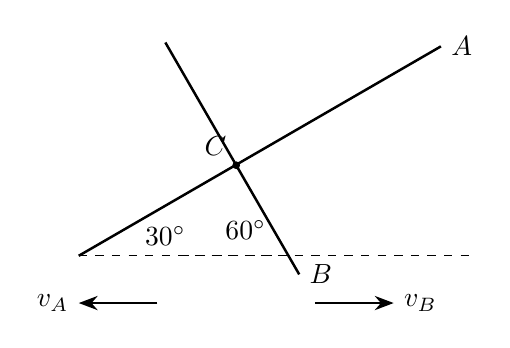
\begin{tikzpicture}\draw[world](-2,-.9)--(2.6,1.76)node[right]{$A$};\draw[world](-.9,1.809)--(.8,-1.136)node[right]{$B$};\fill(0,.25)circle(1.4pt)node[above left]{$C$};\draw[guide](-2,-.9)--(3,-.9);\node at(-.9,-.65){$30^\circ$};\draw[guide](.66,-.9)--(-.7,-.9);\node at(.12,-.57){$60^\circ$};\draw[flow](-1,-1.5)--(-2,-1.5)node[left]{$v_A$};\draw[flow](1,-1.5)--(2,-1.5)node[right]{$v_B$};\end{tikzpicture}
\end{document}
